%%%%%%%%%%%%%%%%%%%%%%%%%%%%%%%%%%%%%%%%%%%%%%%%%%%%%%%%%%%%%%%%%%%%%%%%
%    INSTITUTE OF PHYSICS PUBLISHING                                   %
%                                                                      %
%   `Preparing an article for publication in an Institute of Physics   %
%    Publishing journal using LaTeX'                                   %
%                                                                      %
%    LaTeX source code `ioplau2e.tex' used to generate `author         %
%    guidelines', the documentation explaining and demonstrating use   %
%    of the Institute of Physics Publishing LaTeX preprint files       %
%    `iopart.cls, iopart12.clo and iopart10.clo'.                      %
%                                                                      %
%    `ioplau2e.tex' itself uses LaTeX with `iopart.cls'                %
%                                                                      %
%%%%%%%%%%%%%%%%%%%%%%%%%%%%%%%%%%
%
%
% First we have a character check
%
% ! exclamation mark    " double quote
% # hash                ` opening quote (grave)
% & ampersand           ' closing quote (acute)
% $ dollar              % percent
% ( open parenthesis    ) close paren.
% - hyphen              = equals sign
% | vertical bar        ~ tilde
% @ at sign             _ underscore
% { open curly brace    } close curly
% [ open square         ] close square bracket
% + plus sign           ; semi-colon
% * asterisk            : colon
% < open angle bracket  > close angle
% , comma               . full stop
% ? question mark       / forward slash
% \ backslash           ^ circumflex
%
% ABCDEFGHIJKLMNOPQRSTUVWXYZ
% abcdefghijklmnopqrstuvwxyz
% 1234567890
%
%%%%%%%%%%%%%%%%%%%%%%%%%%%%%%%%%%%%%%%%%%%%%%%%%%%%%%%%%%%%%%%%%%%
%
\documentclass[12pt]{iopart}
\newcommand{\gguide}{{\it Preparing graphics for IOP Publishing journals}}
%Uncomment next line if AMS fonts required
%\usepackage{iopams}
\usepackage{graphicx}
\usepackage{hyperref}   % to set up hyperlinks
\hypersetup{
	colorlinks=true,
	linkcolor=blue,
	citecolor=blue,
	urlcolor=blue,
}

\begin{document}

\note{A novel passive
ferrofluid check (one-way) valve}

% \title{A Novel Passive Ferrofluid One-way (Check) Valve}


%%% first author
\author{Veronica Stuckey$^1$
}
\address{$^1$Biomedical Engineer
}
\ead{stuckey002@gmail.com}
%%% second author
%%% remove the following entry for single author papers
%%% add more entries for additional authors
\author{Robert L. Read$^2$
}

\address{$^2$Public Invention, 1709 Norris Dr., Austin, TX, 78704,
}
\ead{read.robert@gmail.com}
\begin{abstract}

Small pumps and valves enable flow management in microfluidic systems.
A novel passive ferrofluid check valve is presented.
The valve consists of only a
unique channel-and-chamber geometry, ferrofluid, and a stationary
magnetic field.
The flow is determined only by the inlet and output pressure,
and the magnetic field is completely static.
The prototype valve and experimental setup are explained
and performance of the valves cracking and collapse pressure reported.
This initial design can be used for microfluid handling and lab-on-a-chip
applications.
\end{abstract}

%
% Uncomment for keywords
\vspace{2pc}
\noindent{\it Keywords}: ferrofluid, check valve, one-way valve

% Uncomment for Submitted to journal title message
\submitto{\SMS}
%
% Uncomment if a separate title page is required
%\maketitle
%
% For two-column output uncomment the next line and choose [10pt] rather than [12pt] in the \documentclass declaration
%\ioptwocol
%


%%%%%%%%%%%%%%%%%%%%%%%%%%%%%%%%%%%%%%%%%%%%%%%%%%%%%%%%%%%%%%%%%%%%%%
\section{Introduction}

Ferrofluid can be manipulated by electronically controlled magnetic
fields to exert force on fluids\cite{torres2014recent,kole2021engineering,ozbey2015modeling}.
This makes it possible to build pneumatic or hydraulic
devices, perhaps on very small scales,
such as a single chip\cite{yamahata2003ferrofluid,hatch2001ferrofluidic}, to
miniaturize fluid handling.
This has been proposed for biomedical purposes\cite{michelson2019novel}
that would use water or body fluids,
although this paper reports only on experiments done with air.
Miniature pumps and valves could be used to make a “lab on a chip” (LOC) or
even to heat or cool different chip areas.

A fundamental component of such
devices is the {\em check} or one-way valve.
Two check
valves on either side of a chamber whose volume can vary creates a
positive displacement pump.
A perfect check valve opens or
{\em cracks} with minimal pressure on the inlet side and sustains maximal
pressure on the outlet side before {\em collapse},
allowing fluid to flow in only one
direction. Following\cite{hartshorne2004ferrofluid} we call the maximum pressure
differential the valve can resist in the direction it is intended to
check or block (from outlet to inlet) the {\em sustainable} or {\em collapse} pressure.

This article is a brief report on an initial but functioning design of a
passive ferrofluid check valve (PFCV) that has no moving
parts except for the ferrofluid bolus itself, which is stationary
in normal operation.
By passive, the authors
mean a check valve that functions without changes to the magnetic
field affecting the bolus, whether that field is induced by a
permanent magnet or an electromagnet.
That is, the flow is determined
purely by the difference between the inlet port pressure and the
outlet port pressure.
To our knowledge, no passive
ferrofluid check valve has been previously reported, despite being an
active area of research and despite such a valve having
significant advantages for operation and especially
fabrication over valves with moving parts.

%%%%%%%%%%%%%%%%%%%%%%%%%%%%%%%%%%%%%%%%%%%%%%%%%%%%%%%%%%%%%%%%%%%%%%
\section{Related Research}

A number of papers report on ferrofluid pumps, focusing in particular
on micropump and lab-on-a-chip applications\cite{ozbey2015modeling,hsu2018biocompatible}.
Many of these papers use
a version of mechanical valve not based on passive
ferrofluid, even though they move a ferrofluid bolus
with a magnetic field.
For example,
a corrugated silicone micro valve\cite{yamahata2003ferrofluid,yamahata2005plastic}
has been reported.
Other researchers use active valves, which require synchronization with
the ferrofluid plug to form a pump,
such as \cite{menz2000fluidic}, which
describes an active {\em T-Valve} with a moving ferrofluid plug, and
\cite{ando2009ferrofluidic} describes a complete fluid pump with valves
that use
active control of a ferrofluid bolus.
At least two additional kinds of active valves, a {\em well valve} and
{\em Y-valve}, have
been described\cite{hartshorne2004ferrofluid}.
Active control is possible because the
action of the plunger or bolus may be synchronized with the opening and closing
of the valves.
Nonetheless a passive valve would be simpler and less
expensive, and would not require knowledge of the timing of the
plunger.

An interesting functional micropump in which the
moving ferrofluid bolus merges with a fixed ferrofluid valve and then
separates on each pumping cycle has been described\cite{hatch2001ferrofluidic},
but is not a one-way valve.

A passive ferrofluid two-way valve with tunable
opening and closing pressure based on magnetic
field strength\cite{paschalis2013novel} has been tested,
but could not be passively used to make a pump.

This paper has not studied the closing pressure of the PFCV, but reports on
the opening (or cracking) pressure (for flow from inlet to outlet) and
sustainable (or collapse) pressure
when the outlet pressure is higher than the inlet side.

\section{Passive Ferrofluid Check Valve (PFCV) Design}
%%%%%%%%%%%%%%%% begin figure %%%%%%%%%%%%%%%%%%%
%%% 3.34in is the maximum width you can have for a figure
\begin{figure}
\centerline{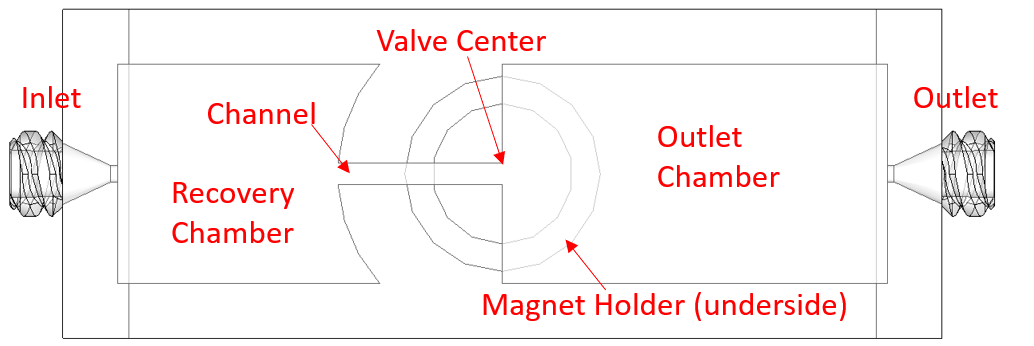
\includegraphics[width=3.34in]{figure/Figure1.png}}
\caption{The passive ferrofluid check valve components}
\label{fig_components}
\end{figure}
%%%%%%%%%%%%%%%% end figure %%%%%%%%%%%%%%%%%%%

The PFCV depicted in Fig.~\ref{fig_components} is a simple asymmetric volume
centered in a magnetic field
which holds a ferrofluid bolus in place.
In the center of a radially symmetric magnetic field
a narrow channel meets a larger open chamber at a right angle.
The ferrofluid bolus is large enough that at rest in the field it
forms a semi-circle in the open chamber. The narrow channel is
longer than the radius of the bolus at rest.
The broad chamber is the outlet side of the valve.
The narrow chamber opens onto a recovery chamber on the inlet
side of the valve.
This design allows the bolus to be recovered from the recovery
chamber when the pressure is equalized if the outlet pressure is
raised above the collapse pressure, driving the bolus away
from the magnetic field.
The PFCV does not resist pressure as well  as a
valve of the same size
made out of moving, solid parts.
That is, the sustainable
pressure it can resist on the outlet side before failing is relatively
low, and pressure required to crack it open and allow flow is
relatively high.
However, it may operate reliably within a range of
known pressures, and thus be sufficient to build a
pump-on-a-chip.
Furthermore, the PFCV reported here is a preliminary design which
can probably be significantly improved.
The authors found the
existence of the PFCV worth sharing immediately.

\section{Method}

The valve depicted Fig.~\ref{fig_components}
was designed using Solidworks 2016.
It is freely licensed via the CERN OHL Strong Reciprocal License\cite{stuckey2021,stuckey2021stl}.
The model consists of a 15mm long, 2mm wide channel, a large outlet
chamber, a recovery chamber,
two female luers, a magnet holder ring and two legs to provide room
for the magnet.  All volumes are 2mm high.
The 3D shape
of the chambers can be thought as a 2mm high extrusion of a 2D shape.
Viewed from the top, one end opens up to a recovery
chamber of circular profile 30mm in diameter and the other
an outlet chamber with a flat wall.
A magnet holder ring 12.7mm inner diameter (1/2'') was created centered on the channel-chamber
junction, below where the bolus is placed, to hold a permanent magnet in place
at the center of the valve. When two magnets are used, the magnet on
top naturally stays in the same position due to attraction to the magnet below.
On the inlet side of the channel
opens into a recovery chamber shaped to allow the ferrofluid to be
passively drawn back into the channel by the magnetic field after a
collapse of the bolus.
The model was printed on a Projet MJP 2500 (3D
Systems, Rock Hill, SC), using Visijet M2G-CL and VisiJet M2 SUP as
material and support respectively (3D Systems, Rock Hill, SC). Support
material was removed by using an EasyClean system (3D Systems, Rock
Hill, SC) and Dawn dish soap (Procter \& Gamble, Cincinnati, OH) to
remove residuals.


%%%%%%%%%%%%%%%% begin figure %%%%%%%%%%%%%%%%%%%
%%% 3.34in is the maximum width you can have for a figure
\begin{figure}
\centerline{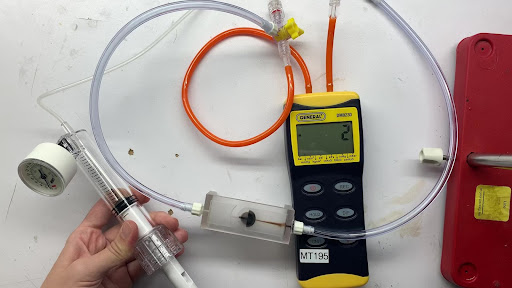
\includegraphics[width=3.34in]{figure/Figure2.jpeg}}
\caption{Equipment set up}
\label{fig_equipment}
\end{figure}
%%%%%%%%%%%%%%%% end figure %%%%%%%%%%%%%%%%%%%

As shown in Fig.~\ref{fig_equipment} and in our demonstration video\cite{stuckey2021video},
a basixCOMPAK 30atm pressurizing syringe (Merit Medical, South Jordan,
UT) is connected to the model via a two-way stopcock (Qosina,
Ronkonkoma, NY), tubing (Natvar, City of Industry, CA), and male
(Injectech, Fort Collins, CO) and female luer (Qosina, Ronkonkoma,
NY), allowing integration of a manometer (General Tools, Secaucus, NJ)
to measure pressure. A 12.7mm x 25.4mm (1/2” x 1”)
cylindrical neodymium magnet (Apex
Magnets, Petersburg, WV) with a pull force of 14.6 kg (32.24 pounds)
was placed inside the magnet channel by means
of a tight fit and 0.2 mL of ferrofluid (Apex Magnets, Petersburg, WV)
was injected into the model using a 3mL syringe (BH Supplies, Jackson,
NJ).

To obtain values, pressure was applied through the pressurizing
syringe, as demonstrated in a video \cite{stuckey2021video}.
Pressure was first applied from the outlet side of the model.
The maximum pressure difference from the outlet side that the
valve can withstand before collapsing, will be referred to as the
sustainable pressure or {\em collapse} pressure.
Pressure applied from the inlet needed to
initiate flow will be referred to as the {\em cracking} pressure.

The cracking pressure was first measured by increasing the pressure
difference on the inlet side until flow is initiated (at which point
the valve is ``open'' and
pushing the syringe plunger faster simply increases flow without
increasing the pressure.) Then the
collapse pressure was measured by increasing the pressure
difference on the outlet side. At pressures below the sustainable
pressure, the valve holds pressure well with no observable leaks of
air in the short time (a few minutes) of our experiment. When the
sustainable pressure is exceeded, the bolus explodes violently into
the recovery chamber. When the pressure difference is equalized, the
bolus may passively recover into the central position, or it may need
to be actively “combed” with a magnet back into the central position.

The procedure was performed first with one magnet, named the “Single
Magnet” configuration, placed below the channel-chamber connection.
The “Dual Magnet” configuration was performed with the magnet in the
same position as the Single Magnet case in the same position, but with
a second magnet of the same kind placed vertically on top of the model,
arranged to be strongly attracted to the lower magnet.

\section{Results}
The final pressures obtained demonstrate a clear difference between
the inlet cracking pressure and outlet sustainable pressure, creating
an effective passive check valve.

\lineup

%%%%%%%%%%%%%%% begin table   %%%%%%%%%%%%%%%%%%%%%%%%%%
\begin{table}[t]
\footnotesize
\caption{\label{table_ASME}Result pressures}
\begin{indented}
\item[]
\begin{tabular}{@{}lllll}
% \begin{tabular}{|p{1.0in} |p{1.0in} |p{1.0in} |p{0.7in} |p{1.0in} |}
\br
 &
Cracking  &
Collapse &
Pressure &
Approx. Ratio: \\
Magnet &
Pressure &
Pressure  &
Difference &
Cracking to \\
configuration &
kPa  (mmHg) &
kPa  (mmHg) &
kPa  (mmHg) &
Collapse Pr. \\
\mr
Single &
1.1 \0(8) &
\05.5 (41) &
4.4 (33) &
1:5 \\
\br
Dual &
8.5 (64) &
17.5 (131)&
8.9 (67)&
1:2 \\
\br
\end{tabular}
\end{indented}
\end{table}
%%%%%%%%%%%%%%%% end table %%%%%%%%%%%%%%%%%%%

The ferrofluid had observable differences in behavior between the two
configurations.  After the pressure equalized
following a collapse of the bolus due to
exceeding the sustainable pressure, the single magnet
configuration often repaired itself by drawing the fluid back
into a centered bolus passively.
After a collapse with two magnets, fluid further from the bolus
remained stationary while the fluid closer was pulled back to the
center. Following the removal of the top magnet, the stationary fluid
then began to return to the bolus. This is consistent with the
localization of the magnetic field between two magnets, and the
weakening of the magnetic field further from the channel-chamber
juncture in the dual magnet configuration.

Although the dual magnet configuration demonstrated a larger absolute
pressure difference due to magnetic field strength between the
cracking and the collapse pressure, the single magnet configuration
granted a larger ratio of collapse pressure to cracking
pressure due to the much lower cracking pressure.
The authors conjecture that the low cracking pressure may have
been not only to the weaker magnetic field, but the weakening at the
top of the 2mm high channel, which was further away from the magnet
in the single magnet configuration.

\section{Conclusions}

This paper demonstrates an apparently novel passive ferrofluid one-way
valve or check valve (PFCV). This valve is completely passive in that
it depends entirely on the pressure at the inlet port and the outlet
port. The valve has no moving parts (except for the ferrofluid, which
is almost stationary), and a remarkably simple design, consisting of
nothing but a channel, an inlet chamber, and outlet chamber,
and a bolus of ferrofluid in a
static magnetic field.

Although no effort has been made to optimize the design, the pressure
difference between the cracking pressure and the sustainable back
pressure appear great enough to make an effective micropump. The
performance of this one-way valve may improve with additional design
effort; the authors sought to publish this result as soon as it was
observed.  Obvious future research possibilities are:
\begin{enumerate}
\item  To improve the
performance by varying the geometry of the passive design or shape and
strength of the magnetic field.
\item Utilizing this design to make a micro-pump
similar to earlier micro-pumps but with this simpler check valve
design.
\item To provide an explanatory and predictive theory of operation,
for example based on magnetic field strength as per \cite{ando2009ferrofluidic}.
\item Studying the ability of the valve to recover after
  a collapse automatically when high outlet pressure is removed,
  which would increase robustness in some applications.
\end{enumerate}

\section{Acknowledgements}

Robert L. Read designed the PFVC. Veronica Stuckey designed, printed,
and tested the model. Both authors contributed to the text of this paper.

\section*{References}

\bibliographystyle{unsrt}
% Here's where you specify the bibliography database file.
% The full file name of the bibliography database for this
% article is asme2e.bib. The name for your database is up
% to you.
\bibliography{ffcv}

\end{document}


‘This is the version of the article before peer review or editing, as submitted by an author to [INSERT NAME OF JOURNAL].  IOP Publishing Ltd is not responsible for any errors or omissions in this version of the manuscript or any version derived from it.  The Version of Record is available online at [INSERT DOI]’ 